
\makeatletter
\def\input@path{{../../}}
\makeatother
\documentclass[../../main.tex]{subfiles}

\graphicspath{
	{../../img/}
	{../img/}
	{img/}
}

\begin{document}
\section{То что диктовал Кастрица}

\subsection{Семейство плоских кривых}

Если кривая задана параметрически:

 \begin{equation} \begin{cases}
 \label{lec18:1}
x=x(t)\\
y=y(t) \\
\alpha \le t \le \beta
\end{cases} k = y'_x = \frac{y'_t}{x'_t} \-- \text{угловой коэффициент 
касательной} \end{equation}

Кривая может быть задана явно:

\begin{equation}\label{lec18:2} F\left( x,y \right)  = 0 \end{equation}

При этом если считать, что $y=y(x)$, то:
\[ y'_x = - \frac{F'_x}{F'_y}\]

Для кривой \eqref{lec18:1} предполагается, что
\[ \left( x' \left( t \right) \right)^2 + \left( y' \left( t \right) \right)^2 
\ne 0, \;  \forall t \in \left[ \alpha, \beta \right] \]

Пусть например $x'\left( t \right) \ne 0 $, тогда в окрестности точки $t_0$ 
функция $f\left( t \right) $ строго монотонна, значит существует обратная 
функция $t\left( x \right) $ и тогда:

\[ y = y \left( t \right) = y \left( t\left( x \right) \right)  \]

Т.~е. в $V \left( t_0 \right) $ эта кривая может быть задана уравнением:
\[ y=y(x) \]

Если же $y'(t_0) \ne 0$, то соответствующим образом получаем, что в $V \left( 
t_0 \right) $ она может быть задана $x=x\left( y \right) $

Рассмотрим уравнение:
\begin{equation} \label{lec18:3} f \left( x,y,c \right) = 0  \end{equation}

Если зафиксировать значение $c$, то мы получаем некоторую кривую вида 
$\eqref{lec18:2}$. Т.~е. $\eqref{lec18:3}$ задает семейство плоских кривых, 
например:

\[ \left( x-c \right)^2 - y = 0 \]

\begin{center} 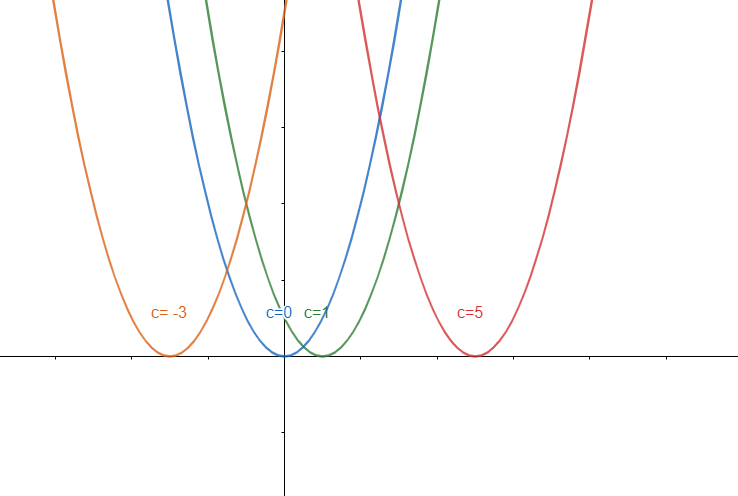
\includegraphics[scale=0.8]{first_family.png} \end{center}


Рассмотрим семейство 

\[ x^2 - y - c = 0 \]

\begin{center} 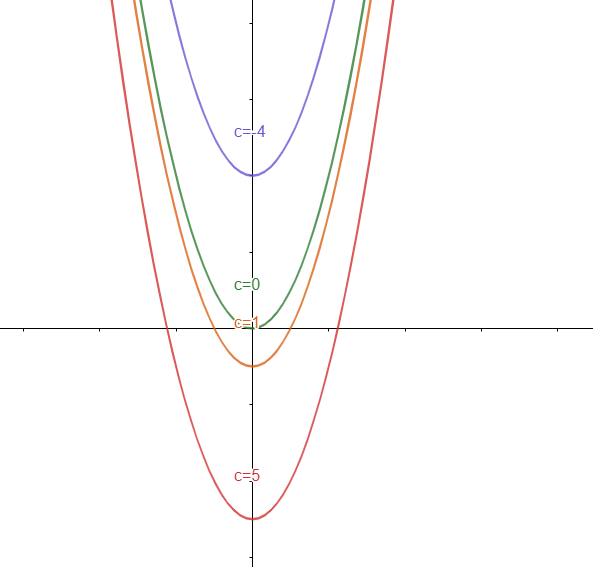
\includegraphics[scale=0.8]{second_family.png} \end{center}


Кривая $\lambda$ называется \emph{ огибающей} семейство кривых 
$\eqref{lec18:3}$, если:

\begin{enumerate}
	\item В каждой точке $\lambda$ касается какой-либо кривой семейства 
	$\eqref{lec18:3}$
	\item $\lambda$ касается всех кривых семейства $\eqref{lec18:3}$
	\item $\lambda$ не имеет общей дуги ни с одной из кривых семейства 
	$\eqref{lec18:3}$
\end{enumerate}

Возьмем какую-либо точку кривой $\lambda$. В этой точке $\lambda$ касается 
некоторой кривой из $\eqref{lec18:3}$, но $\eqref{lec18:3}$ задается по $c$, 
т.~е. точке соответствует параметр $c$, и обратно, при любом $c$, мы получаем 
кривую из $\eqref{lec18:3}$ и соответствующую точку на $\lambda$.

Значит $\lambda$ можно задать параметрическими уравнениями:
\[ \lambda \colon \begin{cases}
x=x\left( c \right) \\
y=y\left( c \right)  
\end{cases} \]

В точке касания касательная имеет угловой коэффициент:
\[ k = \frac{y' \left( c \right) }{ x' \left( c \right) } \]

С другой стороны эта же касательная является касательной и для кривой 
семейства $\eqref{lec18:3} $:
\[ k = - \frac{F'_x}{ F'_y}\] 

приравняв, получаем:

\begin{equation}\label{lec18:4} F'_x x'\left( c \right) + F'_y y'\left( c 
\right) = 0 \end{equation}

Точка $\left( x \left( c\right), y\left( c\right)  \right) $ является точкой, 
соответствующей кривой семейства $\eqref{lec18:3} $ и значит $f \left( x \left( 
c\right), y\left( c\right), c \right) = 0 $

Продифференцируем по $c$:

\begin{equation}\label{lec18:5} F'_x x'\left( c \right) + F'_y y'\left( c 
\right) + F'_c = 0 \end{equation}

Из $\eqref{lec18:4}$ и $\eqref{lec18:5}$, получаем систему:

\begin{equation}\label{lec18:6} \begin{cases}
F'_c \left( x \left( c\right), y\left( c\right), c \right)  = 0\\
F \left( x \left( c\right), y\left( c\right), c \right)  = 0
\end{cases}  \end{equation}

Система $\eqref{lec18:6}$ \--- необходимое условие для огибающей.

Множество точек, удовлетворяющее системе $\eqref{lec18:6}$ называют \emph{ 
дискриминантным множеством} или \emph{ дискриминантной кривой}

Чтобы проверить, что точки задают огибающую кривую в общем случае, нужны 
дополнительные исследования

Рассмотрим примеры:

 \begin{exmp}

\[ \left( x-c\right)^2 - y = 0\]

Составим уравнения вида $\eqref{lec18:6}$:

\[ \begin{cases}
2\left( x-c\right)   = 0\\
\left( x-c\right)^2 - y = 0
\end{cases} \text{откуда} \; y=0 \; \-- \text{уравнение огибающей} \]

\begin{center} 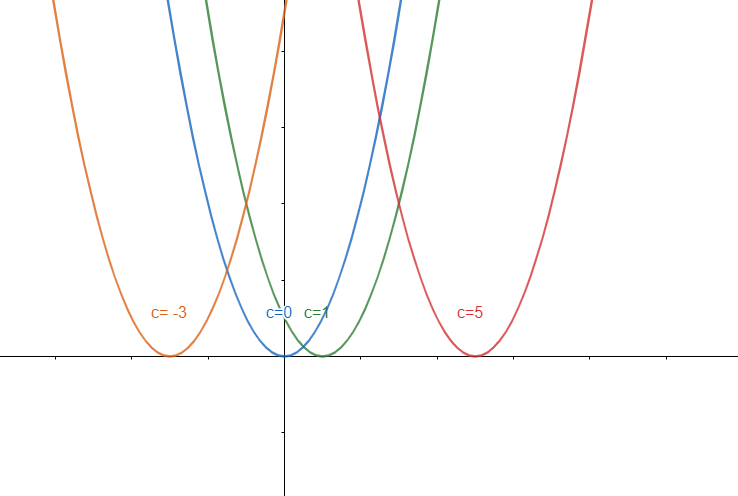
\includegraphics[scale=0.8]{first_family.png} \end{center}


Действительно уравнение $y=0$ задает огибающую семейства $\left( x-c\right)^2 
- y = 0$.
 \end{exmp}

 \begin{exmp}
\[ x^2 - y - c = 0\]

\[ \begin{cases}
-1   = 0\\
x^2 - y - c = 0
\end{cases}  \]
{откуда получаем противоречие $(-1 = 0)$, т.~е. дискриминантное множество 
пустое}
 \end{exmp}

 \begin{exmp}
\[ 3\left( y - c\right)^2 = 2 \left( x-c \right)^3  \]

Составим для этого семейства систему вида $\eqref{lec18:6}$:

\[ \begin{cases}
-6\left( y - c\right)  = -6 \left( x - c\right)^2\\
3\left( y - c\right)^2 = 2 \left( x - c \right)^3
\end{cases}  \]

\[ 3\left( x-c\right)^4  = 2 \left( x-c\right)^3 \]

\[ x-c = \frac{2}{3} \]

Подставляя получаем:

\[ \begin{cases}
y-c  = \frac{4}{9}\\
x-c = \frac{2}{3}
\end{cases}  \]

Откуда:

\[ y - x = -\frac{2}{9} \]

\[ x-c = 0,\ y - c = 0 \]

Т.~е. $y  = x - \frac{2}{9}$, $y=x$. Рассмотрим полученные кривые:

\begin{center} 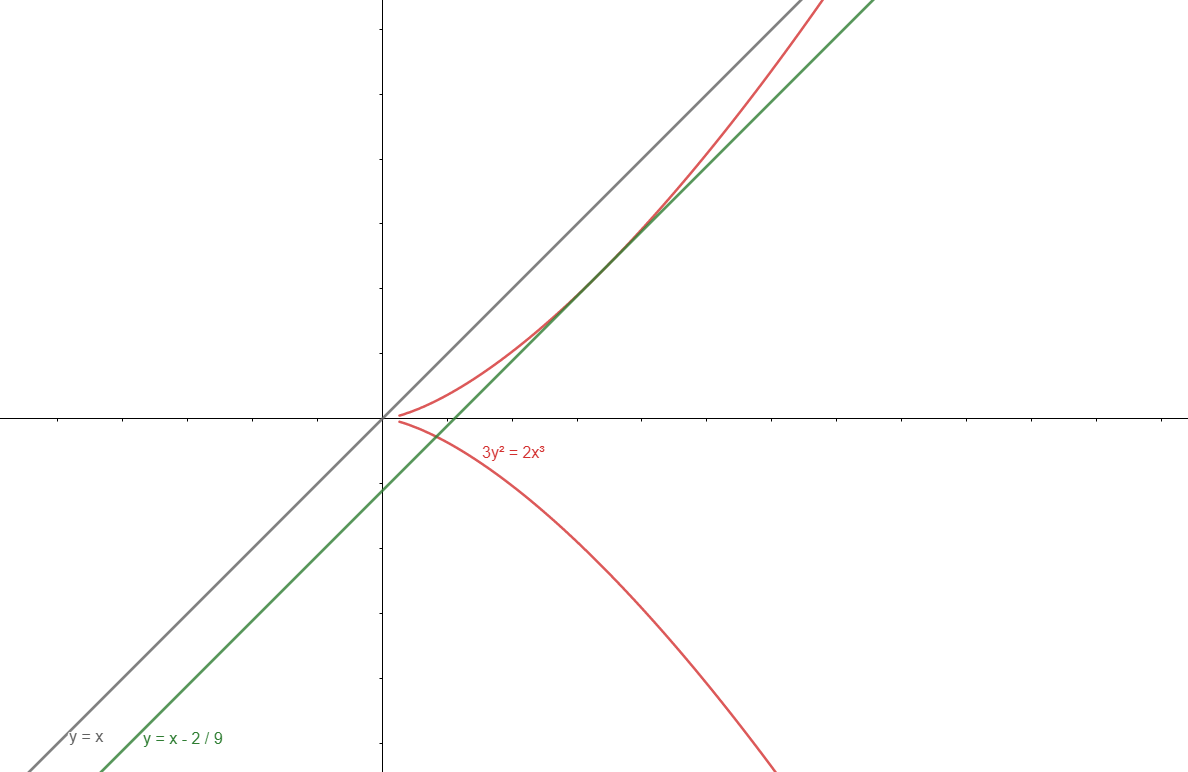
\includegraphics[scale=0.8]{hiperbola.png} \end{center}


Нетрудно видеть, что только $y - x = -\frac{2}{9}$ будет огибающей кривой.

\end{exmp}


\subsection{Криволинейный интеграл 1 рода}

Пусть задана спрямляемая кривая $\overbow{AB}$ и пусть $l$ \--- её длина, на 
ней задано направление из точки $A$ в точку $B$:

\begin{center} 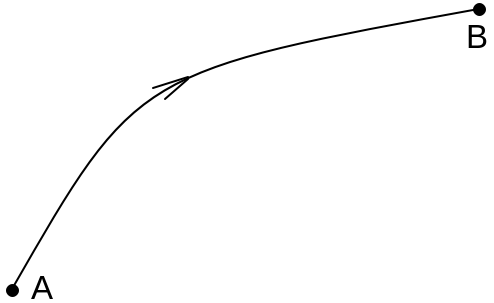
\includegraphics[scale=0.8]{Krivaya1.png} \end{center}


И пусть в точках этой кривой определена функция $f \left( x,y \right) $. 
Рассмотрим разбиение кривой $\overbow{AB}$, точками $A_k,\ k = \overline{0,n}$

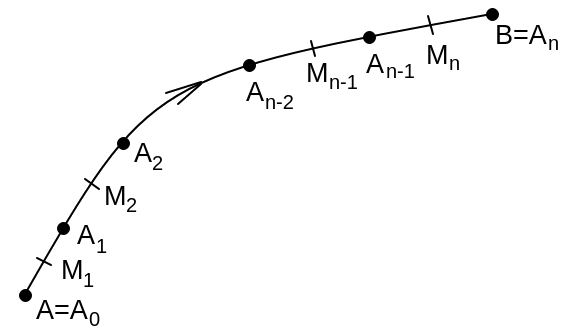
\includegraphics[scale=0.8]{Krivaya2.png}

Обозначим $\Delta S_k$ за длину дуги $\overbow{A_{k-1} A_k}$. $\delta = 
\max_{k} \Delta S_k$ \--- диаметр разбиения.

На каждой дуге $\overbow{A_{k-1} A_k}$ возьмём точку $M_k \left( 
\widetilde{x_k} , \widetilde{y_k} \right) \in \overbow{A_{k-1} A_k}$ и 
построим сумму:

\[ \sigma = \sum_{k=1}^{n} {f \left( \widetilde{x_k} , \widetilde{y_k} \right) 
\Delta S_k}
\]

Такие точки $M_k$ будем называть промежуточными.

Предел $\lim_{\delta \to 0} {\sigma}$ обозначается следующим образом:

\[ \lim_{\delta \to 0} {\sigma} = \int\limits_{ \tiny{\overbow{AB}} }{f\left( 
x,y \right)ds } \]

и называется КрИ-1. 

Если этот предел существует и конечен, т.~е. равен некоторому числу, то 
говорят, что функция $f\left( x,y\right) $ интегрируема на кривой 
$\overbow{AB}$, это будет тогда и только тогда, когда:

\[ \forall \epsilon > 0, \exists \delta_{\epsilon} \colon \forall \delta < 
\delta_{\epsilon} \; \left| \sigma - I \right| < \epsilon  \]

Мы будем предполагать, что функция $f$ ограничена на кривой, а если это не 
так, то конечный предел не будет существовать.

Необходимое условие интегрируемости \--- ограниченность кривой.

\subsection{Геометрический смысл интеграла КрИ-1}

\begin{center} 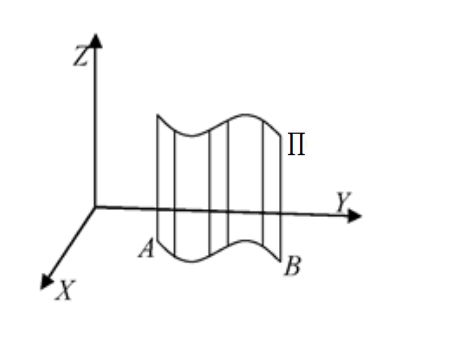
\includegraphics[scale=0.8]{lec18_pi.png} \end{center}


При малом диаметре разбиения $f \left( \widetilde{x_k} , \widetilde{y_k} 
\right) \Delta S_k$ представляет собой диаметр разбиения.

Суммируя элементарные площади, получаем приближенную площадь поверхности $\Pi$

Переходя к пределу, получаем

\[ \int\limits_{ \tiny{\overbow{AB}} }{f\left( x,y \right)ds} = \text{площадь} 
\; \Pi \]

\subsection{Физический смысл интеграла КрИ-1}

На кривой $\overbow{AB}$ рассмотрим плотность в точке $M\left( x,y\right)$, 
$\rho = \rho \left(x,y \right) $, если выделить кусочек $\overbow{A_{k-1} A_k}$

\begin{center} 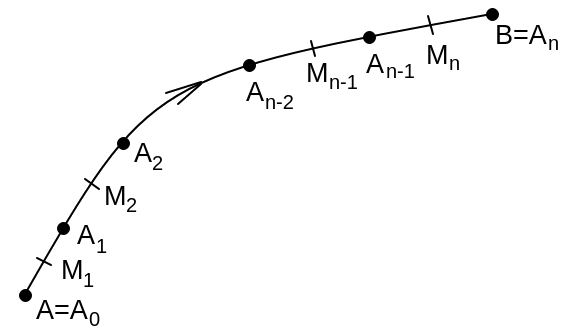
\includegraphics[scale=0.8]{Krivaya2.png} \end{center}


то при достаточно малом разбиении, получаем $\Delta m = \rho \left( 
\widetilde{x_k} , \widetilde{y_k} \right) \Delta S_k$

Суммируя элементарные массы и переходя к пределу, получаем:

\[ \int\limits_{ \tiny{\overbow{AB}} }{f\left( x,y \right)ds} = m = 
\text{масса кривой} \; \overbow{AB}   \]

\subsection{Вычисление КрИ-1}

Пусть кривая $\overbow{AB}$ задана естественной параметризацией: если мы 
зафиксируем $A$, то  $M$  сопоставляется длина дуги  $\overbow{AM}$, т.~е. 

\begin{equation}
\label{lec18:7}
 \begin{cases}
x=x(s)\\
y=y(s) \\
0 \le s \le l
\end{cases}
\end{equation}

Тогда точке $A_k \left( x_k, y_k \right)$ соответствует $S_k$, которая 
порождает $\begin{cases}
x(s_k)\\
y(s_k) 
\end{cases}$

Точке $M_k \left( \widetilde{x_k} , \widetilde{y_k} \right)$ соответствует 
$\widetilde{S_k}$, которая порождает $\begin{cases}
x(\widetilde{s_k})\\
y(\widetilde{s_k}) 
\end{cases}$

Тогда:

\begin{equation}
\label{lec18:8}
\sigma = \sum_{k=1}^{n} f\left( \widetilde{x_k} , \widetilde{y_k} \right) 
\Delta S_k = \sum_{k=1}^{n} f\left( x \left(  \widetilde{s_k} \right)  , y 
\left(  \widetilde{s_k} \right) \right)  \Delta S_k
\end{equation}

Справа интегральная сумма для функции $f\left( x \left( s\right) ,y\left( 
s\right)  \right) $, построенная по разбиению отрезка $\left[ 0,l \right] $, с 
промежуточными точками $\widetilde{s_k}$, это сумма для определенного 
интеграла:

\[ \int_{0}^{l} {f\left( x \left(  \widetilde{s} \right)  , y \left(  
\widetilde{s} \right) \right) ds}\]

Поэтому переходя в $\eqref{lec18:8}$ к пределу, получаем:

\[  \int\limits_{ \tiny{\overbow{AB}} }{f\left( x,y \right)ds} = \int_{0}^{l} 
{f\left( x \left(  \widetilde{s} \right)  , y \left(  \widetilde{s} \right) 
\right) ds} \]

Пусть кривая $\overbow{AB}$ задана произвольной параметризацией:

\[  \begin{cases}
x=x(t)\\
y=y(t) \\
\alpha \le t \le \beta
\end{cases} \]

Точке $A_k \left( x_k,y_k \right) $ соответствует значение параметра $t_k$, 
которое дает $\begin{cases}
x(t_k)\\
y(t_k) 
\end{cases}$

В промежуточной точке $M_k \left( \widetilde{x_k} , \widetilde{y_k} \right) $ 
ей соответствует $\widetilde{t_k}$, а ей соответствует $\begin{cases}
x(\widetilde{t_k})\\
y(\widetilde{t_k}) 
\end{cases}$

$\Delta S_k$ \--- длина дуги $\overbow{A_{k-1}, A_k}$, равна:

\[ \int_{t_{k-1}}^{t_k} {\sqrt{ \left( x' \left( t\right) \right)^2 + \left( 
y' \left( t\right) \right)^2  }} dt
 \]
 
 В силу того, что мы рассматриваем гладкие кривые т.~е. считаем, что $x\left( t 
 \right), y\left( t \right) $ \--- непрерывные, а тогда по теореме о среднем:
 
\[ \exists \overline{t_k} \in \left[ t_{k-1}, t_k \right] \colon \text{длина} 
\; \overbow{A_{k-1}, A_k } = \sqrt{ \left( x' \left( \overline{t_k} \right) 
\right)^2 + \left( y' \left( \overline{t_k} \right) \right)^2 } \Delta t_k    
\]

Т.~к. $\sqrt{ \left( x' \left( t\right) \right)^2 + \left( y' \left( t\right) 
\right)^2  }$ непрерывна на $\left[ \alpha, \beta \right] $ то по Теореме 
Кантора, она равномерно непрерывна на $\left[ \alpha, \beta \right]$, т.~е. ее 
значение при разных разбиениях мало изменится.

\[ \sqrt{ \left( x' \left( \overline{t_k} \right) \right)^2 + \left( y' \left( 
\overline{t_k} \right) \right)^2 } \Delta t_k = \left( \sqrt{ \left( x' \left( 
\widetilde{t_k} \right) \right)^2 + \left( y' \left( \widetilde{t_k} \right) 
\right)^2 } + \alpha_k\right) \Delta t_k \]

\[ \alpha_k = \sqrt{ \left( x' \left( \overline{t_k} \right) \right)^2 + 
\left( y' \left( \overline{t_k} \right) \right)^2 } - \sqrt{ \left( x' \left( 
\widetilde{t_k} \right) \right)^2 + \left( y' \left( \widetilde{t_k} \right) 
\right)^2 } \]

Т.~е. если $\overbow{A_{k-1},A_k}$ достаточно мал, то в двух точках 
$\overline{t_k}$, $\widetilde{t_k}$ будет сколь угодно малой, поскольку 
$\sqrt{ \left( x' \left( t\right) \right)^2 + \left( y' \left( t\right) 
\right)^2  }$ непрерывна на $\left[ \alpha, \beta \right] $, а значит 
равномерно непрерывна на нем, а значит $\alpha_k$ сколь угодно мало. 
Интегральная сумма равна:

\[ \sigma = \sum_{k=1}^{n}{ f\left( \widetilde{x_k} , \widetilde{y_k} \right) 
\sqrt{ \left( x' \left( \widetilde{t_k} \right) \right)^2 + \left( y' \left( 
\widetilde{t_k} \right) \right)^2 } \Delta t_k  } + \sum_{k=1}^{n}{ f\left( 
\widetilde{x_k} , \widetilde{y_k} \right) \alpha_k \Delta t_k} \]

При этом $ \alpha_k \underset{\delta \rightarrow 0}
{\longrightarrow}  0$

Переходя к пределу в интегральной сумме, при $\delta \rightarrow 0$, получаем:

\[ \int\limits_{ \tiny{\overbow{AB}} }{f\left( x,y \right)ds} = 
\int_{\alpha}^{\beta} {f \left( x\left( t\right) , y\left( t\right) \right) 
\sqrt{ \left( x' \left( t \right) \right)^2 + \left( y' \left( t \right) 
\right)^2 } dt} \]

Если кривая задана явно:

\[ \overbow{AB} = \begin{cases} 
y = f\left( x \right) \\
\alpha \le x \le \beta
\end{cases} \]

Тогда ее легко задать параметрически, положив:


\[ \begin{cases} 
x = x \\
y = y \left( x \right) \\
\alpha \le x \le \beta
\end{cases} \]

Исходя из вышеизложенного, будем иметь:

\[ \int\limits_{ \tiny{\overbow{AB}} }{f\left( x,y \right)ds} = 
\int_{\alpha}^{\beta} {f \left( x , y\left( x \right) \right) \sqrt{ 1 + 
\left( y' \left( x \right) \right)^2 } dt} \]

\begin{rem}
КрИ-1 не зависит от выбора направления по кривой $\overbow{AB}$. КрИ-1 
обладает свойствами общими для кратных и определенных интегралов:
\begin{enumerate}
	\item \emph{Линейность}:
	
	\[ \int\limits_{ \tiny{\overbow{AB}} }{\left(  \alpha f + \beta g \right)  \; 
	ds} = \alpha \int\limits_{ \tiny{\overbow{AB}} }{ f \; ds} + \beta 
	\int\limits_{ \tiny{\overbow{AB}} }{ g \; ds} \]
	
	Предполагается, что $f$ и $g$ интегрируемы.
	
	\item \emph{Аддитивность}:
	\[ C \in \overbow{AB} \]
	\[ \int\limits_{ \tiny{\overbow{AB}} }{f  \; ds} = \int\limits_{ 
	\tiny{\overbow{AC}} }{f  \; ds} + \int\limits_{ \tiny{\overbow{CB}} }{f  \; 
	ds} \]
	Предполагается, что $f$ интегрируема.
	
	\item \emph{Монотонность}:
	
	Если для интегрируемых $f$ и $g$ на $\overbow{AB}$ выполняется $f \le g$, то:
	\[ \int\limits_{ \tiny{\overbow{AB}} }{f  \; ds} \le \int\limits_{ 
	\tiny{\overbow{AB}} }{g  \; ds} \]
	
	\item \emph{Монотонность}:
	
	Пусть для интегрируемой $f$ на $\overbow{AB}$ выполняется:
	
	\[ m \le \left| f \left( x,y \right) \right| \le M ,\ \forall \left( x,y 
	\right) \in \overbow{AB}  \]
	Тогда, если обозначить за $l$ длину $\overbow{AB}$, выполняется:
	
	\[ ml \le \int\limits_{ \tiny{\overbow{AB}} }{f  \; ds} \le Ml \]
	
	\item \emph{Теорема о среднем}:
	
	Если $f$ непрерывна на $\overbow{AB}$, то $\exists \left(x_0, y_0 \right) \in 
	\overbow{AB}$, такая, что:
	
	\[ \int\limits_{ \tiny{\overbow{AB}} }{f  \; ds} = f\left( x_0, y_0 \right) l 
	\]
	
\end{enumerate}
	
\end{rem}

Эти свойства вытекают из свойств определенных интегралов, к которым сводится 
КрИ-1.

\begin{exmp}
	Вычислить:
	
	\[ \int\limits_{ \tiny{\overbow{AB}} }{\left( x^2 + xy \right) ds} ,\ 
	\text{где} \; \overbow{AB} \-- \; \text{отрезок} \; A\left( 0,0 \right), 
	B\left( 1,2 \right)   \; \]
	
	\[ \int\limits_{ \tiny{\overbow{AB}} }{\left( x^2 + xy \right) ds} = \left[ 
	\overbow{AB} = \begin{cases} y = 2x \\ 0 \le x \le 1 \end{cases}\right] = 
	\int_{0}^{1} \left( x^2 + 2x^2 \right) \sqrt{1+4} \; dx =  \sqrt{5} \]
	
\end{exmp}

\end{document}
